% automatically generated document using lt2circuiTikz
\documentclass[tikz,margin={2pt 2pt 2pt 2pt}]{standalone}
\usepackage[compatibility,siunitx,  americanvoltages, americancurrents, europeanresistors, europeaninductors, americanports,%
  straightlabels, fetbodydiode, straightvoltages]{circuitikz}
\usepackage{tikz,amsmath, amssymb,bm,color,pgfkeys,siunitx,ifthen,ulem}
\usepackage{pgfplots}
\pgfplotsset{compat=1.14}
\usetikzlibrary{shapes,arrows}
%\usepackage{agaramondc}					% Adobe Garamond, custom shape
%\renewcommand{\shapedefault}{rtl} % rtl: roman tabular lining

\makeatletter

%% bandstop filter (adapted from highpass)
\pgfcircdeclarebipole{}{\ctikzvalof{bipoles/highpass/width}}{*bandstop}{\ctikzvalof{bipoles/highpass/width}}{\ctikzvalof{bipoles/highpass/width}}{
	\pgf@circ@res@step = \ctikzvalof{bipoles/highpass/width}\pgf@circ@Rlen
	\divide \pgf@circ@res@step by 2
	
	\pgfpathmoveto{\pgfpoint{\pgf@circ@res@left}{\pgf@circ@res@zero}}
	\pgf@circ@res@other = \pgf@circ@res@left
	\advance\pgf@circ@res@other by \pgf@circ@res@step 
	
	\ifpgf@circuit@dashed
	\pgfsetdash{{0.1cm}{0.1cm}}{0cm} 
	\fi	
	
	% draw outer box
	\pgfsetlinewidth{\pgfkeysvalueof{/tikz/circuitikz/bipoles/thickness}\pgfstartlinewidth}
	\pgfpathrectanglecorners{\pgfpoint{\pgf@circ@res@left}{\pgf@circ@res@up}}{\pgfpoint{\pgf@circ@res@right}{\pgf@circ@res@down}}
	\pgfusepath{draw}
	
	\ifpgf@circuit@inputarrow
	{
		\advance \pgf@circ@res@left by -.5\pgfkeysvalueof{/tikz/circuitikz/bipoles/thickness}\pgfstartlinewidth
		\pgftransformshift{\pgfpoint{\pgf@circ@res@left}{0pt}}
		\pgfnode{inputarrow}{tip}{}{pgf@inputarrow}{\pgfusepath{fill}}
	}
	\fi
	
	% rotate inner symbol
	\def\pgfcircmathresult{\expandafter\pgf@circ@stripdecimals\pgf@circ@direction\pgf@nil}
	\ifnum \pgfcircmathresult > 45 \ifnum \pgfcircmathresult < 135
	\pgftransformrotate{270}
	\fi\fi
	\ifnum \pgfcircmathresult > 134 \ifnum \pgfcircmathresult < 225  % 134 degree, because >= 135 is not possible
	\pgftransformrotate{180}
	\fi\fi
	\ifnum \pgfcircmathresult > 224 \ifnum \pgfcircmathresult < 315
	\pgftransformrotate{90}
	\fi\fi
	
	% draw inner symbol
	\pgfsetdash{}{0pt}	% always draw solid line for inner symbol
	\pgfsetarrows{-} %never draw arrows
	\pgfsetlinewidth{\pgfstartlinewidth}
	\pgfpathmoveto{\pgfpoint{-0.5\pgf@circ@res@step}{0.5\pgf@circ@res@step}}
	\pgfpathsine{\pgfpoint{.25\pgf@circ@res@step}{.25\pgf@circ@res@step}}
	\pgfpathcosine{\pgfpoint{.25\pgf@circ@res@step}{-.25\pgf@circ@res@step}}
	\pgfpathsine{\pgfpoint{.25\pgf@circ@res@step}{-.25\pgf@circ@res@step}}
	\pgfpathcosine{\pgfpoint{.25\pgf@circ@res@step}{.25\pgf@circ@res@step}}
	\pgfusepath{draw}
	
	\pgfpathmoveto{\pgfpoint{-0.5\pgf@circ@res@step}{0}}
	\pgfpathsine{\pgfpoint{.25\pgf@circ@res@step}{.25\pgf@circ@res@step}}
	\pgfpathcosine{\pgfpoint{.25\pgf@circ@res@step}{-.25\pgf@circ@res@step}}
	\pgfpathsine{\pgfpoint{.25\pgf@circ@res@step}{-.25\pgf@circ@res@step}}
	\pgfpathcosine{\pgfpoint{.25\pgf@circ@res@step}{.25\pgf@circ@res@step}}
	\pgfusepath{draw}
	\pgfpathmoveto{\pgfpoint{-0.15\pgf@circ@res@step}{-0.15\pgf@circ@res@step}}
	\pgfpathlineto{\pgfpoint{0.15\pgf@circ@res@step}{0.15\pgf@circ@res@step}}
	\pgfusepath{draw}
	
	\pgfpathmoveto{\pgfpoint{-0.5\pgf@circ@res@step}{-0.5\pgf@circ@res@step}}
	\pgfpathsine{\pgfpoint{.25\pgf@circ@res@step}{.25\pgf@circ@res@step}}
	\pgfpathcosine{\pgfpoint{.25\pgf@circ@res@step}{-.25\pgf@circ@res@step}}
	\pgfpathsine{\pgfpoint{.25\pgf@circ@res@step}{-.25\pgf@circ@res@step}}
	\pgfpathcosine{\pgfpoint{.25\pgf@circ@res@step}{.25\pgf@circ@res@step}}
	\pgfusepath{draw}
	%	\pgfpathmoveto{\pgfpoint{-0.15\pgf@circ@res@step}{-0.65\pgf@circ@res@step}}
	%	\pgfpathlineto{\pgfpoint{0.15\pgf@circ@res@step}{-0.35\pgf@circ@res@step}}
	%	\pgfusepath{draw}
}

\tikzset{
	*bandstop/.style={\circuitikzbasekey, /tikz/to path=\pgf@circ@*bandstop@path},
}
\def\pgf@circ@*bandstop@path#1{\pgf@circ@bipole@path{*bandstop}{#1}}




\makeatother

\usetikzlibrary{backgrounds,calc,positioning}

\usetikzlibrary{circuits.ee.IEC}
\usetikzlibrary{arrows}


% sym32a style

\ctikzset{tripoles/mos style/arrows}
\ctikzset{
	/tikz/circuitikz/quadpoles/coupler/width=1,%1.3
	/tikz/circuitikz/quadpoles/coupler/height=0.952,%1.3
	/tikz/circuitikz/quadpoles/coupler2/width=1,%1.3
	/tikz/circuitikz/quadpoles/coupler2/height=0.952,%1.3
	/tikz/circuitikz/quadpoles/transformer/width=1.425,%1.5
	/tikz/circuitikz/quadpoles/transformer/height=1.425,%1.5
	/tikz/circuitikz/quadpoles/transformer core/width=1.425,%1.5
	/tikz/circuitikz/quadpoles/transformer core/height=1.425,%1.5
	/tikz/circuitikz/quadpoles/gyrator/width=1.425,%1.5
	/tikz/circuitikz/quadpoles/gyrator/height=1.425,%1.5
	%/tikz/circuitikz/monopoles/tlinestub/width=0.1875,%0.25 no effect!
	/tikz/circuitikz/tripoles/american and port/height=0.95,%.8
	/tikz/circuitikz/tripoles/american nand port/height=0.95,%.8
	/tikz/circuitikz/tripoles/american or port/height=0.95,%.8
	/tikz/circuitikz/tripoles/american nor port/height=0.95,%.8
	/tikz/circuitikz/tripoles/american xor port/height=0.95,%.8
	/tikz/circuitikz/tripoles/american xnor port/height=0.95,%.8
	/tikz/circuitikz/bipoles/tline/height=0.4,%0.3
%	/tikz/circuitikz/bipoles/tline/width=1.2,%0.8
	/tikz/circuitikz/bipoles/diode/height=0.375,%
	/tikz/circuitikz/bipoles/diode/width=0.375,%
	/tikz/circuitikz/bipoles/varcap/height=0.375,%
	/tikz/circuitikz/bipoles/varcap/width=0.375,%
	/tikz/circuitikz/tripoles/triac/height=1.05,%
	/tikz/circuitikz/tripoles/triac/width=0.952,%
	/tikz/circuitikz/tripoles/thyristor/height=1.05,%
	/tikz/circuitikz/tripoles/thyristor/width=0.952,%
	/tikz/circuitikz/tripoles/op amp/height=0.952,%
	/tikz/circuitikz/tripoles/op amp/width=1.2,%
	/tikz/circuitikz/tripoles/op amp/font=\footnotesize,
	/tikz/circuitikz/tripoles/gm amp/height=0.952,% 1.7
	/tikz/circuitikz/tripoles/gm amp/width=1.2,% 1.4
	%	/tikz/circuitikz/tripoles/gm amp/font=\footnotesize,
	/tikz/circuitikz/tripoles/plain amp/height=0.952,% 1.7
	/tikz/circuitikz/tripoles/plain amp/width=1.2,% 1.4
	/tikz/circuitikz/bipoles/resistor/voltage/straight label distance/.initial=.8,
	/tikz/circuitikz/bipoles/generic/voltage/straight label distance/.initial=.8,
	/tikz/circuitikz/bipoles/inductor/voltage/straight label distance/.initial=.8,
	/tikz/circuitikz/bipoles/fullgeneric/voltage/straight label distance/.initial=.8,
	/tikz/circuitikz/bipoles/capacitor/voltage/straight label distance/.initial=1.0,
	/tikz/circuitikz/bipoles/thickness=1.6,
}
\ctikzset{v/.append style={/tikz/european voltages}}

\definecolor{netlabelcolor}{rgb}{0, 0, 0.25}
\definecolor{lttotitextcolor}{rgb}{0, 0.4, 0.25}
\definecolor{lttotidrawcolor}{rgb}{0.6, 0.6, 0.6}
\definecolor{netcolor}{rgb}{0, 0, 0.5}

\pgfkeys{/lt2ti/netlabel/font/.initial= \small}
\pgfkeys{/lt2ti/text/font/.initial= \small}

\pgfkeys{/lt2ti/Net/.style= {netcolor}}
\tikzstyle{dashdotdotted}=[dash pattern=on 3pt off 2pt on \the\pgflinewidth off 2pt on \the\pgflinewidth off 2pt]

\pgfkeys{/lt2ti/VArrow/.style= {->,>=latex}}
\pgfkeys{/lt2ti/SArrow/.style= {->,>=angle 90}}

\begin{document}%
	%\centering%
		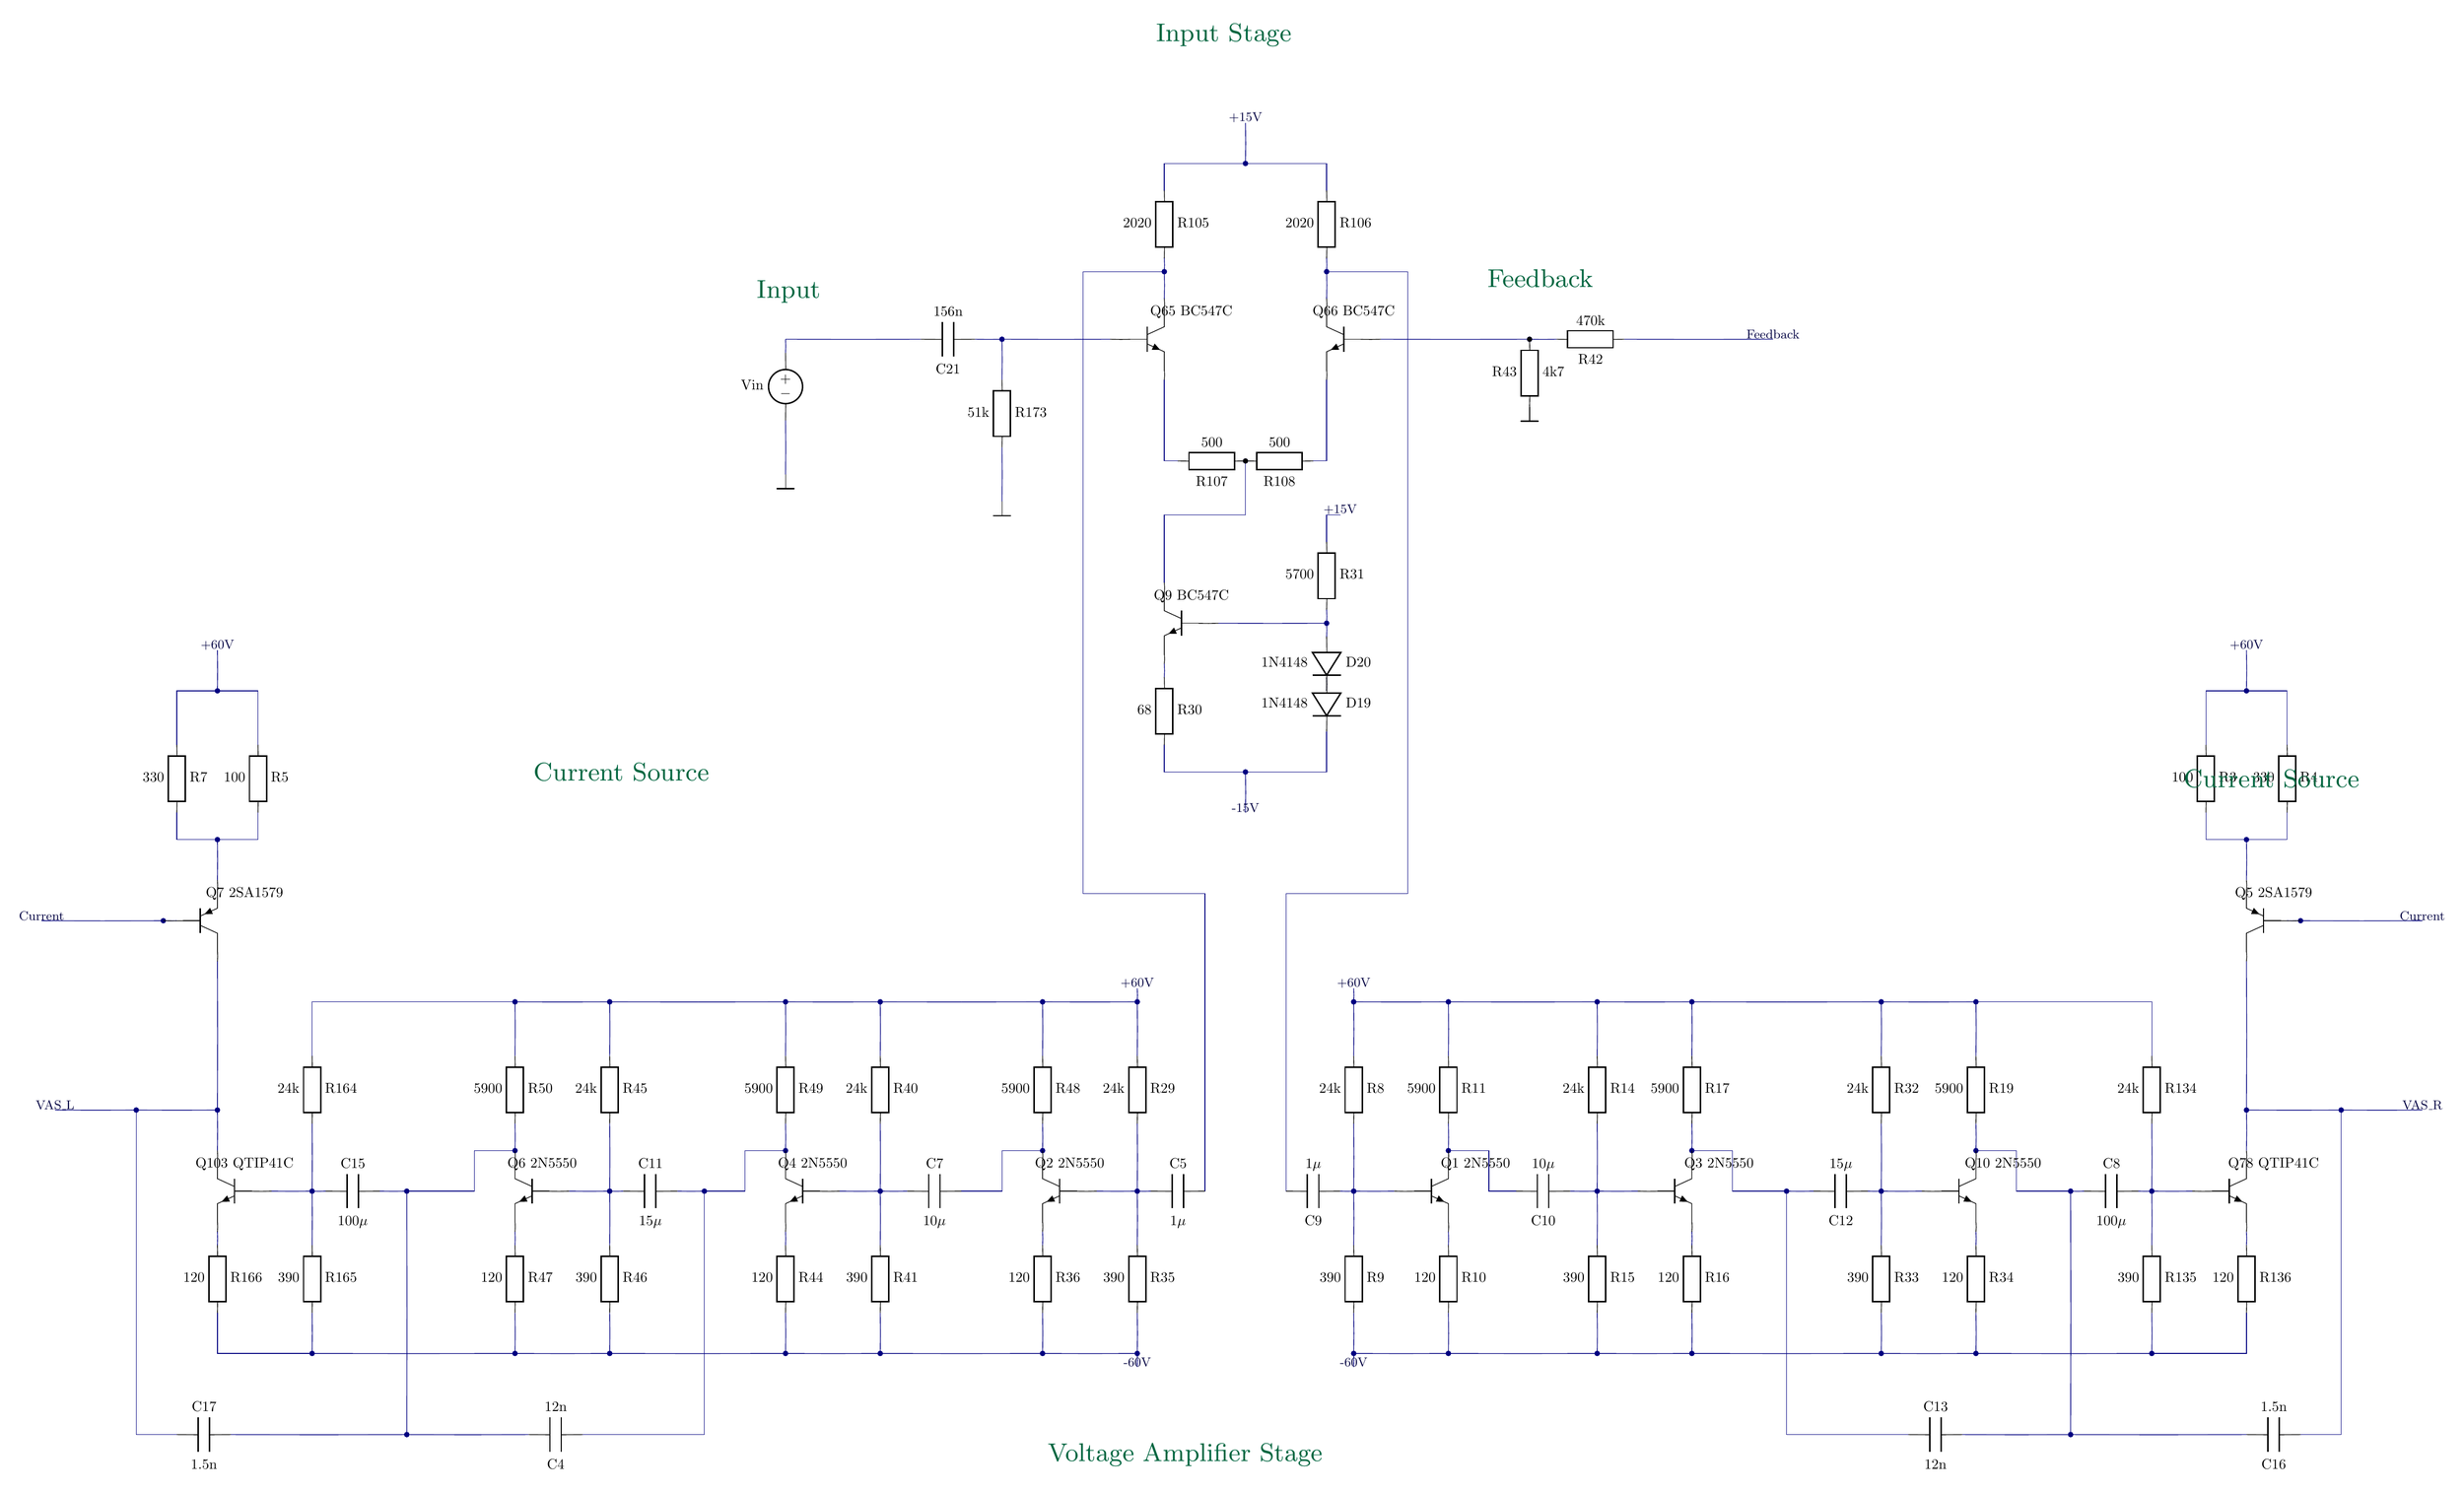
\begin{tikzpicture}[circuit ee IEC, scale=0.6666666667,line width=.5pt]% default: 0.4
	%\tikzstyle{every node}=[font=\small];%
	%\node [draw] at (0.0,0.0) {\pgfkeysvalueof{/tikz/circuitikz/tripoles/op amp/font}};
\draw [/lt2ti/Net](242.5,-137.5)to[*short,*-, color=netcolor] (242.5,-136.0);% wire w3
\draw [/lt2ti/Net](242.5,-137.5)to[*short,*-, color=netcolor] (242.5,-137.5);% wire w4_w6 start
\draw [/lt2ti/Net](239.5,-138.5)to[*short,-, color=netcolor] (239.5,-138.5);% wire w4_w6 end
\draw [/lt2ti/Net](242.5,-137.5) --  (239.5,-137.5) -- (239.5,-138.5); % wire w4_w6 polyline 
\draw [/lt2ti/Net](245.5,-138.5)to[*short,-, color=netcolor] (245.5,-138.5);% wire w5_w7 start
\draw [/lt2ti/Net](242.5,-137.5)to[*short,-*, color=netcolor] (242.5,-137.5);% wire w5_w7 end
\draw [/lt2ti/Net](245.5,-138.5) --  (245.5,-137.5) -- (242.5,-137.5); % wire w5_w7 polyline 
\draw [/lt2ti/Net](239.5,-141.5)to[*short,*-, color=netcolor] (239.5,-141.0);% wire w8
\draw [/lt2ti/Net](245.5,-141.5)to[*short,*-, color=netcolor] (245.5,-141.0);% wire w10
\draw [/lt2ti/Net](239.5,-142.5)to[*short,-*, color=netcolor] (239.5,-141.5);% wire w12
\draw [/lt2ti/Net](245.5,-142.5)to[*short,-*, color=netcolor] (245.5,-141.5);% wire w13
\draw [/lt2ti/Net](230.5,-144.0)to[*short,-, color=netcolor] (225.5,-144.0);% wire w14
\draw [/lt2ti/Net](233.5,-144.0)to[*short,*-, color=netcolor] (232.5,-144.0);% wire w15
\draw [/lt2ti/Net](237.5,-144.0)to[*short,-*, color=netcolor] (233.5,-144.0);% wire w16
\draw [/lt2ti/Net](253.0,-144.0)to[*short,*-, color=netcolor] (247.5,-144.0);% wire w17
\draw [/lt2ti/Net](254.0,-144.0)to[*short,-*, color=netcolor] (253.0,-144.0);% wire w18
\draw [/lt2ti/Net](262.0,-144.0)to[*short,-, color=netcolor] (256.5,-144.0);% wire w19
\draw [/lt2ti/Net](225.5,-144.5)to[*short,-, color=netcolor] (225.5,-144.0);% wire w20
\draw [/lt2ti/Net](233.5,-145.5)to[*short,-*, color=netcolor] (233.5,-144.0);% wire w21
\draw [/lt2ti/Net](240.0,-148.5)to[*short,-, color=netcolor] (240.0,-148.5);% wire w22_w23 start
\draw [/lt2ti/Net](239.5,-145.5)to[*short,-, color=netcolor] (239.5,-145.5);% wire w22_w23 end
\draw [/lt2ti/Net](240.0,-148.5) --  (239.5,-148.5) -- (239.5,-145.5); % wire w22_w23 polyline 
\draw [/lt2ti/Net](245.5,-145.5)to[*short,-, color=netcolor] (245.5,-145.5);% wire w24_w25 start
\draw [/lt2ti/Net](245.0,-148.5)to[*short,-, color=netcolor] (245.0,-148.5);% wire w24_w25 end
\draw [/lt2ti/Net](245.5,-145.5) --  (245.5,-148.5) -- (245.0,-148.5); % wire w24_w25 polyline 
\draw [/lt2ti/Net](225.5,-149.0)to[*short,-, color=netcolor] (225.5,-147.0);% wire w26
\draw [/lt2ti/Net](233.5,-150.0)to[*short,-, color=netcolor] (233.5,-148.0);% wire w27
\draw [/lt2ti/Net](246.0,-150.5)to[*short,-, color=netcolor] (246.0,-150.5);% wire w30_w31 start
\draw [/lt2ti/Net](245.5,-151.5)to[*short,-, color=netcolor] (245.5,-151.5);% wire w30_w31 end
\draw [/lt2ti/Net](246.0,-150.5) --  (245.5,-150.5) -- (245.5,-151.5); % wire w30_w31 polyline 
\draw [/lt2ti/Net](239.5,-153.0)to[*short,-, color=netcolor] (239.5,-153.0);% wire w32_w28_w29 start
\draw [/lt2ti/Net](242.5,-148.5)to[*short,-*, color=netcolor] (242.5,-148.5);% wire w32_w28_w29 end
\draw [/lt2ti/Net](239.5,-153.0) --  (239.5,-150.5) --  (242.5,-150.5) -- (242.5,-148.5); % wire w32_w28_w29 polyline 
\draw [/lt2ti/Net](245.5,-154.5)to[*short,*-, color=netcolor] (245.5,-154.0);% wire w33
\draw [/lt2ti/Net](245.5,-154.5)to[*short,*-, color=netcolor] (241.5,-154.5);% wire w34
\draw [/lt2ti/Net](245.5,-155.0)to[*short,-*, color=netcolor] (245.5,-154.5);% wire w35
\draw [/lt2ti/Net](239.5,-156.5)to[*short,-, color=netcolor] (239.5,-156.0);% wire w36
\draw [/lt2ti/Net](204.5,-157.0)to[*short,*-, color=netcolor] (204.5,-155.5);% wire w37
\draw [/lt2ti/Net](204.5,-157.0)to[*short,*-, color=netcolor] (204.5,-157.0);% wire w38_w44 start
\draw [/lt2ti/Net](203.0,-159.0)to[*short,-, color=netcolor] (203.0,-159.0);% wire w38_w44 end
\draw [/lt2ti/Net](204.5,-157.0) --  (203.0,-157.0) -- (203.0,-159.0); % wire w38_w44 polyline 
\draw [/lt2ti/Net](245.5,-157.0)to[*short,-, color=netcolor] (245.5,-156.5);% wire w40
\draw [/lt2ti/Net](279.5,-157.0)to[*short,*-, color=netcolor] (279.5,-155.5);% wire w41
\draw [/lt2ti/Net](279.5,-157.0)to[*short,*-, color=netcolor] (279.5,-157.0);% wire w42_w46 start
\draw [/lt2ti/Net](278.0,-159.0)to[*short,-, color=netcolor] (278.0,-159.0);% wire w42_w46 end
\draw [/lt2ti/Net](279.5,-157.0) --  (278.0,-157.0) -- (278.0,-159.0); % wire w42_w46 polyline 
\draw [/lt2ti/Net](206.0,-159.0)to[*short,-, color=netcolor] (206.0,-159.0);% wire w39_w45 start
\draw [/lt2ti/Net](204.5,-157.0)to[*short,-*, color=netcolor] (204.5,-157.0);% wire w39_w45 end
\draw [/lt2ti/Net](206.0,-159.0) --  (206.0,-157.0) -- (204.5,-157.0); % wire w39_w45 polyline 
\draw [/lt2ti/Net](281.0,-159.0)to[*short,-, color=netcolor] (281.0,-159.0);% wire w43_w47 start
\draw [/lt2ti/Net](279.5,-157.0)to[*short,-*, color=netcolor] (279.5,-157.0);% wire w43_w47 end
\draw [/lt2ti/Net](281.0,-159.0) --  (281.0,-157.0) -- (279.5,-157.0); % wire w43_w47 polyline 
\draw [/lt2ti/Net](242.5,-160.0)to[*short,*-, color=netcolor] (242.5,-160.0);% wire w48_w49 start
\draw [/lt2ti/Net](239.5,-159.0)to[*short,-, color=netcolor] (239.5,-159.0);% wire w48_w49 end
\draw [/lt2ti/Net](242.5,-160.0) --  (239.5,-160.0) -- (239.5,-159.0); % wire w48_w49 polyline 
\draw [/lt2ti/Net](245.5,-158.5)to[*short,-, color=netcolor] (245.5,-158.5);% wire w50_w51 start
\draw [/lt2ti/Net](242.5,-160.0)to[*short,-*, color=netcolor] (242.5,-160.0);% wire w50_w51 end
\draw [/lt2ti/Net](245.5,-158.5) --  (245.5,-160.0) -- (242.5,-160.0); % wire w50_w51 polyline 
\draw [/lt2ti/Net](242.5,-161.5)to[*short,-*, color=netcolor] (242.5,-160.0);% wire w52
\draw [/lt2ti/Net](204.5,-162.5)to[*short,*-, color=netcolor] (204.5,-162.5);% wire w53_w54 start
\draw [/lt2ti/Net](203.0,-161.5)to[*short,-, color=netcolor] (203.0,-161.5);% wire w53_w54 end
\draw [/lt2ti/Net](204.5,-162.5) --  (203.0,-162.5) -- (203.0,-161.5); % wire w53_w54 polyline 
\draw [/lt2ti/Net](206.0,-161.5)to[*short,-, color=netcolor] (206.0,-161.5);% wire w55_w56 start
\draw [/lt2ti/Net](204.5,-162.5)to[*short,-*, color=netcolor] (204.5,-162.5);% wire w55_w56 end
\draw [/lt2ti/Net](206.0,-161.5) --  (206.0,-162.5) -- (204.5,-162.5); % wire w55_w56 polyline 
\draw [/lt2ti/Net](279.5,-162.5)to[*short,*-, color=netcolor] (279.5,-162.5);% wire w57_w58 start
\draw [/lt2ti/Net](278.0,-161.5)to[*short,-, color=netcolor] (278.0,-161.5);% wire w57_w58 end
\draw [/lt2ti/Net](279.5,-162.5) --  (278.0,-162.5) -- (278.0,-161.5); % wire w57_w58 polyline 
\draw [/lt2ti/Net](281.0,-161.5)to[*short,-, color=netcolor] (281.0,-161.5);% wire w59_w60 start
\draw [/lt2ti/Net](279.5,-162.5)to[*short,-*, color=netcolor] (279.5,-162.5);% wire w59_w60 end
\draw [/lt2ti/Net](281.0,-161.5) --  (281.0,-162.5) -- (279.5,-162.5); % wire w59_w60 polyline 
\draw [/lt2ti/Net](204.5,-164.0)to[*short,-*, color=netcolor] (204.5,-162.5);% wire w61
\draw [/lt2ti/Net](279.5,-164.0)to[*short,-*, color=netcolor] (279.5,-162.5);% wire w62
\draw [/lt2ti/Net](202.5,-165.5)to[*short,*-, color=netcolor] (198.0,-165.5);% wire w67
\draw [/lt2ti/Net](203.0,-165.5)to[*short,-*, color=netcolor] (202.5,-165.5);% wire w68
\draw [/lt2ti/Net](281.5,-165.5)to[*short,*-, color=netcolor] (281.0,-165.5);% wire w69
\draw [/lt2ti/Net](286.0,-165.5)to[*short,-*, color=netcolor] (281.5,-165.5);% wire w70
\draw [/lt2ti/Net](215.5,-168.5)to[*short,*-, color=netcolor] (215.5,-168.5);% wire w71_w85 start
\draw [/lt2ti/Net](208.0,-170.5)to[*short,-, color=netcolor] (208.0,-170.5);% wire w71_w85 end
\draw [/lt2ti/Net](215.5,-168.5) --  (208.0,-168.5) -- (208.0,-170.5); % wire w71_w85 polyline 
\draw [/lt2ti/Net](219.0,-168.5)to[*short,*-*, color=netcolor] (215.5,-168.5);% wire w72
\draw [/lt2ti/Net](225.5,-168.5)to[*short,*-*, color=netcolor] (219.0,-168.5);% wire w73
\draw [/lt2ti/Net](229.0,-168.5)to[*short,*-*, color=netcolor] (225.5,-168.5);% wire w74
\draw [/lt2ti/Net](235.0,-168.5)to[*short,*-*, color=netcolor] (229.0,-168.5);% wire w75
\draw [/lt2ti/Net](238.5,-168.5)to[*short,*-, color=netcolor] (238.5,-168.0);% wire w76
\draw [/lt2ti/Net](238.5,-168.5)to[*short,*-*, color=netcolor] (235.0,-168.5);% wire w77
\draw [/lt2ti/Net](246.5,-168.5)to[*short,*-, color=netcolor] (246.5,-168.0);% wire w78
\draw [/lt2ti/Net](250.0,-168.5)to[*short,*-*, color=netcolor] (246.5,-168.5);% wire w79
\draw [/lt2ti/Net](255.5,-168.5)to[*short,*-*, color=netcolor] (250.0,-168.5);% wire w80
\draw [/lt2ti/Net](259.0,-168.5)to[*short,*-*, color=netcolor] (255.5,-168.5);% wire w81
\draw [/lt2ti/Net](266.0,-168.5)to[*short,*-*, color=netcolor] (259.0,-168.5);% wire w82
\draw [/lt2ti/Net](269.5,-168.5)to[*short,*-*, color=netcolor] (266.0,-168.5);% wire w83
\draw [/lt2ti/Net](215.5,-170.5)to[*short,-*, color=netcolor] (215.5,-168.5);% wire w86
\draw [/lt2ti/Net](219.0,-170.5)to[*short,-*, color=netcolor] (219.0,-168.5);% wire w87
\draw [/lt2ti/Net](225.5,-170.5)to[*short,-*, color=netcolor] (225.5,-168.5);% wire w88
\draw [/lt2ti/Net](229.0,-170.5)to[*short,-*, color=netcolor] (229.0,-168.5);% wire w89
\draw [/lt2ti/Net](235.0,-170.5)to[*short,-*, color=netcolor] (235.0,-168.5);% wire w90
\draw [/lt2ti/Net](238.5,-170.5)to[*short,-*, color=netcolor] (238.5,-168.5);% wire w91
\draw [/lt2ti/Net](246.5,-170.5)to[*short,-*, color=netcolor] (246.5,-168.5);% wire w92
\draw [/lt2ti/Net](250.0,-170.5)to[*short,-*, color=netcolor] (250.0,-168.5);% wire w93
\draw [/lt2ti/Net](255.5,-170.5)to[*short,-*, color=netcolor] (255.5,-168.5);% wire w94
\draw [/lt2ti/Net](259.0,-170.5)to[*short,-*, color=netcolor] (259.0,-168.5);% wire w95
\draw [/lt2ti/Net](266.0,-170.5)to[*short,-*, color=netcolor] (266.0,-168.5);% wire w96
\draw [/lt2ti/Net](269.5,-170.5)to[*short,-*, color=netcolor] (269.5,-168.5);% wire w97
\draw [/lt2ti/Net](276.0,-170.5)to[*short,-, color=netcolor] (276.0,-170.5);% wire w84_w98 start
\draw [/lt2ti/Net](269.5,-168.5)to[*short,-*, color=netcolor] (269.5,-168.5);% wire w84_w98 end
\draw [/lt2ti/Net](276.0,-170.5) --  (276.0,-168.5) -- (269.5,-168.5); % wire w84_w98 polyline 
\draw [/lt2ti/Net](201.5,-172.5)to[*short,*-, color=netcolor] (198.5,-172.5);% wire w99
\draw [/lt2ti/Net](204.5,-172.5)to[*short,*-, color=netcolor] (204.5,-167.0);% wire w100
\draw [/lt2ti/Net](204.5,-172.5)to[*short,*-*, color=netcolor] (201.5,-172.5);% wire w101
\draw [/lt2ti/Net](279.5,-172.5)to[*short,*-, color=netcolor] (279.5,-167.0);% wire w102
\draw [/lt2ti/Net](283.0,-172.5)to[*short,*-*, color=netcolor] (279.5,-172.5);% wire w103
\draw [/lt2ti/Net](283.0,-172.5)to[*short,*-, color=netcolor] (283.0,-172.5);% wire w221_w222 start
\draw [/lt2ti/Net](281.5,-184.5)to[*short,-, color=netcolor] (281.5,-184.5);% wire w221_w222 end
\draw [/lt2ti/Net](283.0,-172.5) --  (283.0,-184.5) -- (281.5,-184.5); % wire w221_w222 polyline 
\draw [/lt2ti/Net](286.0,-172.5)to[*short,-*, color=netcolor] (283.0,-172.5);% wire w104
\draw [/lt2ti/Net](204.5,-174.0)to[*short,-*, color=netcolor] (204.5,-172.5);% wire w105
\draw [/lt2ti/Net](215.5,-174.0)to[*short,*-, color=netcolor] (215.5,-173.0);% wire w106
\draw [/lt2ti/Net](215.5,-174.0)to[*short,*-, color=netcolor] (215.5,-174.0);% wire w124_w107_w123 start
\draw [/lt2ti/Net](211.5,-175.5)to[*short,-*, color=netcolor] (211.5,-175.5);% wire w124_w107_w123 end
\draw [/lt2ti/Net](215.5,-174.0) --  (214.0,-174.0) --  (214.0,-175.5) -- (211.5,-175.5); % wire w124_w107_w123 polyline 
\draw [/lt2ti/Net](225.5,-174.0)to[*short,*-, color=netcolor] (225.5,-173.0);% wire w108
\draw [/lt2ti/Net](225.5,-174.0)to[*short,*-, color=netcolor] (225.5,-174.0);% wire w130_w109_w129 start
\draw [/lt2ti/Net](222.5,-175.5)to[*short,-*, color=netcolor] (222.5,-175.5);% wire w130_w109_w129 end
\draw [/lt2ti/Net](225.5,-174.0) --  (224.0,-174.0) --  (224.0,-175.5) -- (222.5,-175.5); % wire w130_w109_w129 polyline 
\draw [/lt2ti/Net](235.0,-174.0)to[*short,*-, color=netcolor] (235.0,-173.0);% wire w110
\draw [/lt2ti/Net](235.0,-174.0)to[*short,*-, color=netcolor] (235.0,-174.0);% wire w135_w111_w134 start
\draw [/lt2ti/Net](232.0,-175.5)to[*short,-, color=netcolor] (232.0,-175.5);% wire w135_w111_w134 end
\draw [/lt2ti/Net](235.0,-174.0) --  (233.5,-174.0) --  (233.5,-175.5) -- (232.0,-175.5); % wire w135_w111_w134 polyline 
\draw [/lt2ti/Net](250.0,-174.0)to[*short,*-, color=netcolor] (250.0,-173.0);% wire w112
\draw [/lt2ti/Net](259.0,-174.0)to[*short,*-, color=netcolor] (259.0,-173.0);% wire w114
\draw [/lt2ti/Net](269.5,-174.0)to[*short,*-, color=netcolor] (269.5,-173.0);% wire w116
\draw [/lt2ti/Net](279.5,-174.0)to[*short,-*, color=netcolor] (279.5,-172.5);% wire w118
\draw [/lt2ti/Net](208.0,-175.5)to[*short,*-, color=netcolor] (208.0,-173.0);% wire w119
\draw [/lt2ti/Net](208.0,-175.5)to[*short,*-, color=netcolor] (206.5,-175.5);% wire w120
\draw [/lt2ti/Net](208.5,-175.5)to[*short,-*, color=netcolor] (208.0,-175.5);% wire w121
\draw [/lt2ti/Net](211.5,-175.5)to[*short,*-, color=netcolor] (210.5,-175.5);% wire w122
\draw [/lt2ti/Net](219.0,-175.5)to[*short,*-, color=netcolor] (219.0,-173.0);% wire w125
\draw [/lt2ti/Net](219.0,-175.5)to[*short,*-, color=netcolor] (217.5,-175.5);% wire w126
\draw [/lt2ti/Net](219.5,-175.5)to[*short,-*, color=netcolor] (219.0,-175.5);% wire w127
\draw [/lt2ti/Net](222.5,-175.5)to[*short,*-, color=netcolor] (221.5,-175.5);% wire w128
\draw [/lt2ti/Net](222.5,-175.5)to[*short,*-, color=netcolor] (222.5,-175.5);% wire w214_w215 start
\draw [/lt2ti/Net](218.0,-184.5)to[*short,-, color=netcolor] (218.0,-184.5);% wire w214_w215 end
\draw [/lt2ti/Net](222.5,-175.5) --  (222.5,-184.5) -- (218.0,-184.5); % wire w214_w215 polyline 
\draw [/lt2ti/Net](229.0,-175.5)to[*short,*-, color=netcolor] (229.0,-173.0);% wire w131
\draw [/lt2ti/Net](229.0,-175.5)to[*short,*-, color=netcolor] (227.5,-175.5);% wire w132
\draw [/lt2ti/Net](230.0,-175.5)to[*short,-*, color=netcolor] (229.0,-175.5);% wire w133
\draw [/lt2ti/Net](238.5,-175.5)to[*short,*-, color=netcolor] (238.5,-173.0);% wire w136
\draw [/lt2ti/Net](238.5,-175.5)to[*short,*-, color=netcolor] (237.0,-175.5);% wire w137
\draw [/lt2ti/Net](239.0,-175.5)to[*short,-*, color=netcolor] (238.5,-175.5);% wire w138
\draw [/lt2ti/Net](241.0,-175.5)to[*short,-, color=netcolor] (241.0,-175.5);% wire w139_w64_w9_w63 start
\draw [/lt2ti/Net](239.5,-141.5)to[*short,-*, color=netcolor] (239.5,-141.5);% wire w139_w64_w9_w63 end
\draw [/lt2ti/Net](241.0,-175.5) --  (241.0,-164.5) --  (236.5,-164.5) --  (236.5,-141.5) -- (239.5,-141.5); % wire w139_w64_w9_w63 polyline 
\draw [/lt2ti/Net](244.0,-175.5)to[*short,-, color=netcolor] (244.0,-175.5);% wire w140_w66_w11_w65 start
\draw [/lt2ti/Net](245.5,-141.5)to[*short,-*, color=netcolor] (245.5,-141.5);% wire w140_w66_w11_w65 end
\draw [/lt2ti/Net](244.0,-175.5) --  (244.0,-164.5) --  (248.5,-164.5) --  (248.5,-141.5) -- (245.5,-141.5); % wire w140_w66_w11_w65 polyline 
\draw [/lt2ti/Net](246.5,-175.5)to[*short,*-, color=netcolor] (246.5,-173.0);% wire w141
\draw [/lt2ti/Net](246.5,-175.5)to[*short,*-, color=netcolor] (246.0,-175.5);% wire w142
\draw [/lt2ti/Net](248.0,-175.5)to[*short,-*, color=netcolor] (246.5,-175.5);% wire w143
\draw [/lt2ti/Net](252.5,-175.5)to[*short,-, color=netcolor] (252.5,-175.5);% wire w145_w113_w144 start
\draw [/lt2ti/Net](250.0,-174.0)to[*short,-*, color=netcolor] (250.0,-174.0);% wire w145_w113_w144 end
\draw [/lt2ti/Net](252.5,-175.5) --  (251.5,-175.5) --  (251.5,-174.0) -- (250.0,-174.0); % wire w145_w113_w144 polyline 
\draw [/lt2ti/Net](255.5,-175.5)to[*short,*-, color=netcolor] (255.5,-173.0);% wire w146
\draw [/lt2ti/Net](255.5,-175.5)to[*short,*-, color=netcolor] (254.5,-175.5);% wire w147
\draw [/lt2ti/Net](257.0,-175.5)to[*short,-*, color=netcolor] (255.5,-175.5);% wire w148
\draw [/lt2ti/Net](262.5,-175.5)to[*short,*-, color=netcolor] (262.5,-175.5);% wire w150_w115_w149 start
\draw [/lt2ti/Net](259.0,-174.0)to[*short,-*, color=netcolor] (259.0,-174.0);% wire w150_w115_w149 end
\draw [/lt2ti/Net](262.5,-175.5) --  (260.5,-175.5) --  (260.5,-174.0) -- (259.0,-174.0); % wire w150_w115_w149 polyline 
\draw [/lt2ti/Net](263.5,-175.5)to[*short,-*, color=netcolor] (262.5,-175.5);% wire w151
\draw [/lt2ti/Net](266.0,-175.5)to[*short,*-, color=netcolor] (266.0,-173.0);% wire w152
\draw [/lt2ti/Net](266.0,-175.5)to[*short,*-, color=netcolor] (265.5,-175.5);% wire w153
\draw [/lt2ti/Net](267.5,-175.5)to[*short,-*, color=netcolor] (266.0,-175.5);% wire w154
\draw [/lt2ti/Net](273.0,-175.5)to[*short,*-, color=netcolor] (273.0,-175.5);% wire w156_w117_w155 start
\draw [/lt2ti/Net](269.5,-174.0)to[*short,-*, color=netcolor] (269.5,-174.0);% wire w156_w117_w155 end
\draw [/lt2ti/Net](273.0,-175.5) --  (271.0,-175.5) --  (271.0,-174.0) -- (269.5,-174.0); % wire w156_w117_w155 polyline 
\draw [/lt2ti/Net](273.5,-175.5)to[*short,-*, color=netcolor] (273.0,-175.5);% wire w157
\draw [/lt2ti/Net](276.0,-175.5)to[*short,*-, color=netcolor] (276.0,-173.0);% wire w158
\draw [/lt2ti/Net](276.0,-175.5)to[*short,*-, color=netcolor] (275.5,-175.5);% wire w159
\draw [/lt2ti/Net](277.5,-175.5)to[*short,-*, color=netcolor] (276.0,-175.5);% wire w160
\draw [/lt2ti/Net](204.5,-177.5)to[*short,-, color=netcolor] (204.5,-177.0);% wire w161
\draw [/lt2ti/Net](208.0,-177.5)to[*short,-*, color=netcolor] (208.0,-175.5);% wire w162
\draw [/lt2ti/Net](215.5,-177.5)to[*short,-, color=netcolor] (215.5,-177.0);% wire w163
\draw [/lt2ti/Net](219.0,-177.5)to[*short,-*, color=netcolor] (219.0,-175.5);% wire w164
\draw [/lt2ti/Net](225.5,-177.5)to[*short,-, color=netcolor] (225.5,-177.0);% wire w165
\draw [/lt2ti/Net](229.0,-177.5)to[*short,-*, color=netcolor] (229.0,-175.5);% wire w166
\draw [/lt2ti/Net](235.0,-177.5)to[*short,-, color=netcolor] (235.0,-177.0);% wire w167
\draw [/lt2ti/Net](238.5,-177.5)to[*short,-*, color=netcolor] (238.5,-175.5);% wire w168
\draw [/lt2ti/Net](246.5,-177.5)to[*short,-*, color=netcolor] (246.5,-175.5);% wire w169
\draw [/lt2ti/Net](250.0,-177.5)to[*short,-, color=netcolor] (250.0,-177.0);% wire w170
\draw [/lt2ti/Net](255.5,-177.5)to[*short,-*, color=netcolor] (255.5,-175.5);% wire w171
\draw [/lt2ti/Net](259.0,-177.5)to[*short,-, color=netcolor] (259.0,-177.0);% wire w172
\draw [/lt2ti/Net](266.0,-177.5)to[*short,-*, color=netcolor] (266.0,-175.5);% wire w173
\draw [/lt2ti/Net](269.5,-177.5)to[*short,-, color=netcolor] (269.5,-177.0);% wire w174
\draw [/lt2ti/Net](276.0,-177.5)to[*short,-*, color=netcolor] (276.0,-175.5);% wire w175
\draw [/lt2ti/Net](279.5,-177.5)to[*short,-, color=netcolor] (279.5,-177.0);% wire w176
\draw [/lt2ti/Net](208.0,-181.5)to[*short,*-, color=netcolor] (208.0,-180.0);% wire w178
\draw [/lt2ti/Net](208.0,-181.5)to[*short,*-, color=netcolor] (208.0,-181.5);% wire w177_w179 start
\draw [/lt2ti/Net](204.5,-180.0)to[*short,-, color=netcolor] (204.5,-180.0);% wire w177_w179 end
\draw [/lt2ti/Net](208.0,-181.5) --  (204.5,-181.5) -- (204.5,-180.0); % wire w177_w179 polyline 
\draw [/lt2ti/Net](215.5,-181.5)to[*short,*-, color=netcolor] (215.5,-180.0);% wire w180
\draw [/lt2ti/Net](215.5,-181.5)to[*short,*-*, color=netcolor] (208.0,-181.5);% wire w181
\draw [/lt2ti/Net](219.0,-181.5)to[*short,*-, color=netcolor] (219.0,-180.0);% wire w182
\draw [/lt2ti/Net](219.0,-181.5)to[*short,*-*, color=netcolor] (215.5,-181.5);% wire w183
\draw [/lt2ti/Net](225.5,-181.5)to[*short,*-, color=netcolor] (225.5,-180.0);% wire w184
\draw [/lt2ti/Net](225.5,-181.5)to[*short,*-*, color=netcolor] (219.0,-181.5);% wire w185
\draw [/lt2ti/Net](229.0,-181.5)to[*short,*-, color=netcolor] (229.0,-180.0);% wire w186
\draw [/lt2ti/Net](229.0,-181.5)to[*short,*-*, color=netcolor] (225.5,-181.5);% wire w187
\draw [/lt2ti/Net](235.0,-181.5)to[*short,*-, color=netcolor] (235.0,-180.0);% wire w188
\draw [/lt2ti/Net](235.0,-181.5)to[*short,*-*, color=netcolor] (229.0,-181.5);% wire w189
\draw [/lt2ti/Net](238.5,-181.5)to[*short,*-, color=netcolor] (238.5,-180.0);% wire w190
\draw [/lt2ti/Net](238.5,-181.5)to[*short,*-*, color=netcolor] (235.0,-181.5);% wire w191
\draw [/lt2ti/Net](246.5,-181.5)to[*short,*-, color=netcolor] (246.5,-180.0);% wire w192
\draw [/lt2ti/Net](250.0,-181.5)to[*short,*-, color=netcolor] (250.0,-180.0);% wire w193
\draw [/lt2ti/Net](250.0,-181.5)to[*short,*-*, color=netcolor] (246.5,-181.5);% wire w194
\draw [/lt2ti/Net](255.5,-181.5)to[*short,*-, color=netcolor] (255.5,-180.0);% wire w195
\draw [/lt2ti/Net](255.5,-181.5)to[*short,*-*, color=netcolor] (250.0,-181.5);% wire w196
\draw [/lt2ti/Net](259.0,-181.5)to[*short,*-, color=netcolor] (259.0,-180.0);% wire w197
\draw [/lt2ti/Net](259.0,-181.5)to[*short,*-*, color=netcolor] (255.5,-181.5);% wire w198
\draw [/lt2ti/Net](266.0,-181.5)to[*short,*-, color=netcolor] (266.0,-180.0);% wire w199
\draw [/lt2ti/Net](266.0,-181.5)to[*short,*-*, color=netcolor] (259.0,-181.5);% wire w200
\draw [/lt2ti/Net](269.5,-181.5)to[*short,*-, color=netcolor] (269.5,-180.0);% wire w201
\draw [/lt2ti/Net](269.5,-181.5)to[*short,*-*, color=netcolor] (266.0,-181.5);% wire w202
\draw [/lt2ti/Net](276.0,-181.5)to[*short,*-, color=netcolor] (276.0,-180.0);% wire w203
\draw [/lt2ti/Net](276.0,-181.5)to[*short,*-*, color=netcolor] (269.5,-181.5);% wire w204
\draw [/lt2ti/Net](279.5,-180.0)to[*short,-, color=netcolor] (279.5,-180.0);% wire w205_w206 start
\draw [/lt2ti/Net](276.0,-181.5)to[*short,-*, color=netcolor] (276.0,-181.5);% wire w205_w206 end
\draw [/lt2ti/Net](279.5,-180.0) --  (279.5,-181.5) -- (276.0,-181.5); % wire w205_w206 polyline 
\draw [/lt2ti/Net](238.5,-182.0)to[*short,-*, color=netcolor] (238.5,-181.5);% wire w207
\draw [/lt2ti/Net](246.5,-182.0)to[*short,-*, color=netcolor] (246.5,-181.5);% wire w208
\draw [/lt2ti/Net](203.0,-184.5)to[*short,-, color=netcolor] (203.0,-184.5);% wire w209_w210 start
\draw [/lt2ti/Net](201.5,-172.5)to[*short,-*, color=netcolor] (201.5,-172.5);% wire w209_w210 end
\draw [/lt2ti/Net](203.0,-184.5) --  (201.5,-184.5) -- (201.5,-172.5); % wire w209_w210 polyline 
\draw [/lt2ti/Net](211.5,-184.5)to[*short,*-*, color=netcolor] (211.5,-175.5);% wire w211
\draw [/lt2ti/Net](211.5,-184.5)to[*short,*-, color=netcolor] (205.0,-184.5);% wire w212
\draw [/lt2ti/Net](216.0,-184.5)to[*short,-*, color=netcolor] (211.5,-184.5);% wire w213
\draw [/lt2ti/Net](267.0,-184.5)to[*short,-, color=netcolor] (267.0,-184.5);% wire w216_w217 start
\draw [/lt2ti/Net](262.5,-175.5)to[*short,-*, color=netcolor] (262.5,-175.5);% wire w216_w217 end
\draw [/lt2ti/Net](267.0,-184.5) --  (262.5,-184.5) -- (262.5,-175.5); % wire w216_w217 polyline 
\draw [/lt2ti/Net](273.0,-184.5)to[*short,*-*, color=netcolor] (273.0,-175.5);% wire w218
\draw [/lt2ti/Net](273.0,-184.5)to[*short,*-, color=netcolor] (269.0,-184.5);% wire w219
\draw [/lt2ti/Net](279.5,-184.5)to[*short,-*, color=netcolor] (273.0,-184.5);% wire w220
 \draw (225.5, -149.0) node[rground, xscale=1, yscale=1, rotate=0, ] (undefined) {};%  (undefined)++(0.0,0.0) node {undefined }; % component "circuiTikz\gnd" "undefined" 
 \draw (233.5, -150.0) node[rground, xscale=1, yscale=1, rotate=0, ] (undefined) {};%  (undefined)++(0.0,0.0) node {undefined }; % component "circuiTikz\gnd" "undefined" 
 \draw (253.0, -146.5) node[rground, xscale=1, yscale=1, rotate=0, ] (undefined) {};%  (undefined)++(0.0,0.0) node {undefined }; % component "circuiTikz\gnd" "undefined" 
 \draw (239.5, -144.0) node[npn, nobodydiode, , rotate=0, ] (Q65) {}   (Q65)++(1.0,1) node {Q65 BC547C}; % component "npn" "Q65" 
 \draw (237.5, -144.0) to [*short, -] (Q65.B); \draw (239.5, -145.5) to [*short, -] (Q65.E); \draw (239.5, -142.5) to [*short, -] (Q65.C);% extend wires to the connection points   % component "npn" "Q65" 
 \draw (245.5, -144.0) node[npn, nobodydiode, xscale=-1, rotate=0, ] (Q66) {}   (Q66)++(1.0,1) node {Q66 BC547C}; % component "npn" "Q66" 
 \draw (247.5, -144.0) to [*short, -] (Q66.B); \draw (245.5, -145.5) to [*short, -] (Q66.E); \draw (245.5, -142.5) to [*short, -] (Q66.C);% extend wires to the connection points   % component "npn" "Q66" 
  \draw (239.5, -138.5) to[*resistor, l^=R105, a_=2020, -, ] (239.5,-141.0){}; %\node [] at (239.0,-138.0) {x}; % component "res" "R105" 
  \draw (245.5, -138.5) to[*resistor, l^=R106, a_=2020, -, ] (245.5,-141.0){}; %\node [] at (246.0,-138.0) {x}; % component "res" "R106" 
  \draw (242.5, -148.5) to[*resistor, l^=R107, a_=500, *-, ] (240.0,-148.5){}; %\node [] at (243.0,-148.0) {x}; % component "res" "R107" 
  \draw (245.0, -148.5) to[*resistor, l^=R108, a_=500, -, ] (242.5,-148.5){}; %\node [] at (245.5,-148.0) {x}; % component "res" "R108" 
  \draw (276.0, -170.5) to[*resistor, l^=R134, a_=24k, -, ] (276.0,-173.0){}; %\node [] at (275.5,-170.0) {x}; % component "res" "R134" 
  \draw (276.0, -177.5) to[*resistor, l^=R135, a_=390, -, ] (276.0,-180.0){}; %\node [] at (275.5,-177.0) {x}; % component "res" "R135" 
 \draw (279.5, -175.5) node[npn, nobodydiode, , rotate=0, ] (Q78) {}   (Q78)++(1.0,1) node {Q78 QTIP41C}; % component "npn" "Q78" 
 \draw (277.5, -175.5) to [*short, -] (Q78.B); \draw (279.5, -177.0) to [*short, -] (Q78.E); \draw (279.5, -174.0) to [*short, -] (Q78.C);% extend wires to the connection points   % component "npn" "Q78" 
  \draw (279.5, -177.5) to[*resistor, l^=R136, a_=120, -, ] (279.5,-180.0){}; %\node [] at (279.0,-177.0) {x}; % component "res" "R136" 
  \draw (281.5, -184.5) to[*capacitor, l^=C16, a_=1.5n, -, ] (279.5,-184.5){}; % component "cap" "C16" 
  %\node [] at (281.5,-184.0) {x}; % component "cap" "C16" 
  \draw (208.0, -170.5) to[*resistor, l^=R164, a_=24k, -, ] (208.0,-173.0){}; %\node [] at (208.5,-170.0) {x}; % component "res" "R164" 
  \draw (208.0, -177.5) to[*resistor, l^=R165, a_=390, -, ] (208.0,-180.0){}; %\node [] at (208.5,-177.0) {x}; % component "res" "R165" 
 \draw (204.5, -175.5) node[npn, nobodydiode, xscale=-1, rotate=0, ] (Q103) {}   (Q103)++(1.0,1) node {Q103 QTIP41C}; % component "npn" "Q103" 
 \draw (206.5, -175.5) to [*short, -] (Q103.B); \draw (204.5, -177.0) to [*short, -] (Q103.E); \draw (204.5, -174.0) to [*short, -] (Q103.C);% extend wires to the connection points   % component "npn" "Q103" 
  \draw (204.5, -177.5) to[*resistor, l^=R166, a_=120, -, ] (204.5,-180.0){}; %\node [] at (205.0,-177.0) {x}; % component "res" "R166" 
  \draw (203.0, -184.5) to[*capacitor, l^=C17, a_=1.5n, -, ] (205.0,-184.5){}; % component "cap" "C17" 
  %\node [] at (203.0,-184.0) {x}; % component "cap" "C17" 
  \draw (225.5, -144.5) to[*V, l_=Vin] (225.5,-147.0){}; % component "voltage" "V4" 
  \draw (232.5, -144.0) to[*capacitor, l^=C21, a_=156n, -, ] (230.5,-144.0){}; % component "cap" "C21" 
  %\node [] at (232.5,-143.5) {x}; % component "cap" "C21" 
  \draw (233.5, -145.5) to[*resistor, l^=R173, a_=51k, -, ] (233.5,-148.0){}; %\node [] at (234.0,-145.0) {x}; % component "res" "R173" 
  \draw (245.5, -156.5) to[*diode, l^=D19, a_=1N4148, ] (245.5,-158.5){}; % component "diode" "D19" 
  \draw (245.5, -155.0) to[*diode, l^=D20, a_=1N4148, ] (245.5,-157.0){}; % component "diode" "D20" 
 \draw (239.5, -154.5) node[npn, nobodydiode, xscale=-1, rotate=0, ] (Q9) {}   (Q9)++(1.0,1) node {Q9 BC547C}; % component "npn" "Q9" 
 \draw (241.5, -154.5) to [*short, -] (Q9.B); \draw (239.5, -156.0) to [*short, -] (Q9.E); \draw (239.5, -153.0) to [*short, -] (Q9.C);% extend wires to the connection points   % component "npn" "Q9" 
  \draw (239.5, -156.5) to[*resistor, l^=R30, a_=68, -, ] (239.5,-159.0){}; %\node [] at (239.0,-156.0) {x}; % component "res" "R30" 
  \draw (245.5, -151.5) to[*resistor, l^=R31, a_=5700, -, ] (245.5,-154.0){}; %\node [] at (245.0,-151.0) {x}; % component "res" "R31" 
  \draw (246.5, -170.5) to[*resistor, l^=R8, a_=24k, -, ] (246.5,-173.0){}; %\node [] at (246.0,-170.0) {x}; % component "res" "R8" 
  \draw (246.5, -177.5) to[*resistor, l^=R9, a_=390, -, ] (246.5,-180.0){}; %\node [] at (246.0,-177.0) {x}; % component "res" "R9" 
 \draw (250.0, -175.5) node[npn, nobodydiode, , rotate=0, ] (Q1) {}   (Q1)++(1.0,1) node {Q1 2N5550}; % component "npn" "Q1" 
 \draw (248.0, -175.5) to [*short, -] (Q1.B); \draw (250.0, -177.0) to [*short, -] (Q1.E); \draw (250.0, -174.0) to [*short, -] (Q1.C);% extend wires to the connection points   % component "npn" "Q1" 
  \draw (250.0, -177.5) to[*resistor, l^=R10, a_=120, -, ] (250.0,-180.0){}; %\node [] at (249.5,-177.0) {x}; % component "res" "R10" 
  \draw (255.5, -170.5) to[*resistor, l^=R14, a_=24k, -, ] (255.5,-173.0){}; %\node [] at (255.0,-170.0) {x}; % component "res" "R14" 
  \draw (255.5, -177.5) to[*resistor, l^=R15, a_=390, -, ] (255.5,-180.0){}; %\node [] at (255.0,-177.0) {x}; % component "res" "R15" 
 \draw (259.0, -175.5) node[npn, nobodydiode, , rotate=0, ] (Q3) {}   (Q3)++(1.0,1) node {Q3 2N5550}; % component "npn" "Q3" 
 \draw (257.0, -175.5) to [*short, -] (Q3.B); \draw (259.0, -177.0) to [*short, -] (Q3.E); \draw (259.0, -174.0) to [*short, -] (Q3.C);% extend wires to the connection points   % component "npn" "Q3" 
  \draw (259.0, -177.5) to[*resistor, l^=R16, a_=120, -, ] (259.0,-180.0){}; %\node [] at (258.5,-177.0) {x}; % component "res" "R16" 
  \draw (266.0, -170.5) to[*resistor, l^=R32, a_=24k, -, ] (266.0,-173.0){}; %\node [] at (265.5,-170.0) {x}; % component "res" "R32" 
  \draw (266.0, -177.5) to[*resistor, l^=R33, a_=390, -, ] (266.0,-180.0){}; %\node [] at (265.5,-177.0) {x}; % component "res" "R33" 
 \draw (269.5, -175.5) node[npn, nobodydiode, , rotate=0, ] (Q10) {}   (Q10)++(1.0,1) node {Q10 2N5550}; % component "npn" "Q10" 
 \draw (267.5, -175.5) to [*short, -] (Q10.B); \draw (269.5, -177.0) to [*short, -] (Q10.E); \draw (269.5, -174.0) to [*short, -] (Q10.C);% extend wires to the connection points   % component "npn" "Q10" 
  \draw (269.5, -177.5) to[*resistor, l^=R34, a_=120, -, ] (269.5,-180.0){}; %\node [] at (269.0,-177.0) {x}; % component "res" "R34" 
  \draw (256.5, -144.0) to[*resistor, l^=R42, a_=470k, -, ] (254.0,-144.0){}; %\node [] at (257.0,-143.5) {x}; % component "res" "R42" 
  \draw (253.0, -146.5) to[*resistor, l^=R43, a_=4k7, -*, ] (253.0,-144.0){}; %\node [] at (253.5,-147.0) {x}; % component "res" "R43" 
  \draw (250.0, -170.5) to[*resistor, l^=R11, a_=5900, -, ] (250.0,-173.0){}; %\node [] at (249.5,-170.0) {x}; % component "res" "R11" 
  \draw (259.0, -170.5) to[*resistor, l^=R17, a_=5900, -, ] (259.0,-173.0){}; %\node [] at (258.5,-170.0) {x}; % component "res" "R17" 
  \draw (269.5, -170.5) to[*resistor, l^=R19, a_=5900, -, ] (269.5,-173.0){}; %\node [] at (269.0,-170.0) {x}; % component "res" "R19" 
  \draw (267.0, -184.5) to[*capacitor, l^=C13, a_=12n, -, ] (269.0,-184.5){}; % component "cap" "C13" 
  %\node [] at (267.0,-184.0) {x}; % component "cap" "C13" 
  \draw (273.5, -175.5) to[*capacitor, l^=C8, a_=100$\mu$, -, ] (275.5,-175.5){}; % component "cap" "C8" 
  %\node [] at (273.5,-175.0) {x}; % component "cap" "C8" 
  \draw (208.5, -175.5) to[*capacitor, l^=C15, a_=100$\mu$, -, ] (210.5,-175.5){}; % component "cap" "C15" 
  %\node [] at (208.5,-175.0) {x}; % component "cap" "C15" 
  \draw (246.0, -175.5) to[*capacitor, l^=C9, a_=1$\mu$, -, ] (244.0,-175.5){}; % component "cap" "C9" 
  %\node [] at (246.0,-175.0) {x}; % component "cap" "C9" 
  \draw (254.5, -175.5) to[*capacitor, l^=C10, a_=10$\mu$, -, ] (252.5,-175.5){}; % component "cap" "C10" 
  %\node [] at (254.5,-175.0) {x}; % component "cap" "C10" 
  \draw (265.5, -175.5) to[*capacitor, l^=C12, a_=15$\mu$, -, ] (263.5,-175.5){}; % component "cap" "C12" 
  %\node [] at (265.5,-175.0) {x}; % component "cap" "C12" 
  \draw (238.5, -170.5) to[*resistor, l^=R29, a_=24k, -, ] (238.5,-173.0){}; %\node [] at (239.0,-170.0) {x}; % component "res" "R29" 
  \draw (238.5, -177.5) to[*resistor, l^=R35, a_=390, -, ] (238.5,-180.0){}; %\node [] at (239.0,-177.0) {x}; % component "res" "R35" 
 \draw (235.0, -175.5) node[npn, nobodydiode, xscale=-1, rotate=0, ] (Q2) {}   (Q2)++(1.0,1) node {Q2 2N5550}; % component "npn" "Q2" 
 \draw (237.0, -175.5) to [*short, -] (Q2.B); \draw (235.0, -177.0) to [*short, -] (Q2.E); \draw (235.0, -174.0) to [*short, -] (Q2.C);% extend wires to the connection points   % component "npn" "Q2" 
  \draw (235.0, -177.5) to[*resistor, l^=R36, a_=120, -, ] (235.0,-180.0){}; %\node [] at (235.5,-177.0) {x}; % component "res" "R36" 
  \draw (229.0, -170.5) to[*resistor, l^=R40, a_=24k, -, ] (229.0,-173.0){}; %\node [] at (229.5,-170.0) {x}; % component "res" "R40" 
  \draw (229.0, -177.5) to[*resistor, l^=R41, a_=390, -, ] (229.0,-180.0){}; %\node [] at (229.5,-177.0) {x}; % component "res" "R41" 
 \draw (225.5, -175.5) node[npn, nobodydiode, xscale=-1, rotate=0, ] (Q4) {}   (Q4)++(1.0,1) node {Q4 2N5550}; % component "npn" "Q4" 
 \draw (227.5, -175.5) to [*short, -] (Q4.B); \draw (225.5, -177.0) to [*short, -] (Q4.E); \draw (225.5, -174.0) to [*short, -] (Q4.C);% extend wires to the connection points   % component "npn" "Q4" 
  \draw (225.5, -177.5) to[*resistor, l^=R44, a_=120, -, ] (225.5,-180.0){}; %\node [] at (226.0,-177.0) {x}; % component "res" "R44" 
  \draw (219.0, -170.5) to[*resistor, l^=R45, a_=24k, -, ] (219.0,-173.0){}; %\node [] at (219.5,-170.0) {x}; % component "res" "R45" 
  \draw (219.0, -177.5) to[*resistor, l^=R46, a_=390, -, ] (219.0,-180.0){}; %\node [] at (219.5,-177.0) {x}; % component "res" "R46" 
 \draw (215.5, -175.5) node[npn, nobodydiode, xscale=-1, rotate=0, ] (Q6) {}   (Q6)++(1.0,1) node {Q6 2N5550}; % component "npn" "Q6" 
 \draw (217.5, -175.5) to [*short, -] (Q6.B); \draw (215.5, -177.0) to [*short, -] (Q6.E); \draw (215.5, -174.0) to [*short, -] (Q6.C);% extend wires to the connection points   % component "npn" "Q6" 
  \draw (215.5, -177.5) to[*resistor, l^=R47, a_=120, -, ] (215.5,-180.0){}; %\node [] at (216.0,-177.0) {x}; % component "res" "R47" 
  \draw (235.0, -170.5) to[*resistor, l^=R48, a_=5900, -, ] (235.0,-173.0){}; %\node [] at (235.5,-170.0) {x}; % component "res" "R48" 
  \draw (225.5, -170.5) to[*resistor, l^=R49, a_=5900, -, ] (225.5,-173.0){}; %\node [] at (226.0,-170.0) {x}; % component "res" "R49" 
  \draw (215.5, -170.5) to[*resistor, l^=R50, a_=5900, -, ] (215.5,-173.0){}; %\node [] at (216.0,-170.0) {x}; % component "res" "R50" 
  \draw (218.0, -184.5) to[*capacitor, l^=C4, a_=12n, -, ] (216.0,-184.5){}; % component "cap" "C4" 
  %\node [] at (218.0,-184.0) {x}; % component "cap" "C4" 
  \draw (239.0, -175.5) to[*capacitor, l^=C5, a_=1$\mu$, -, ] (241.0,-175.5){}; % component "cap" "C5" 
  %\node [] at (239.0,-175.0) {x}; % component "cap" "C5" 
  \draw (230.0, -175.5) to[*capacitor, l^=C7, a_=10$\mu$, -, ] (232.0,-175.5){}; % component "cap" "C7" 
  %\node [] at (230.0,-175.0) {x}; % component "cap" "C7" 
  \draw (219.5, -175.5) to[*capacitor, l^=C11, a_=15$\mu$, -, ] (221.5,-175.5){}; % component "cap" "C11" 
  %\node [] at (219.5,-175.0) {x}; % component "cap" "C11" 
 \draw (279.5, -165.5) node[pnp, nobodydiode, xscale=-1, yscale=1, rotate=-360, ] (Q5) {}   (Q5)++(1.0,1) node {Q5 2SA1579}; % component "pnp" "Q5" 
 \draw (281.5, -165.5) to [*short, -] (Q5.B); \draw (279.5, -164.0) to [*short, -] (Q5.E); \draw (279.5, -167.0) to [*short, -] (Q5.C);% extend wires to the connection points   % component "pnp" "Q5" 
  \draw (278.0, -159.0) to[*resistor, l^=R3, a_=100, -, ] (278.0,-161.5){}; %\node [] at (277.5,-158.5) {x}; % component "res" "R3" 
  \draw (281.0, -159.0) to[*resistor, l^=R4, a_=330, -, ] (281.0,-161.5){}; %\node [] at (280.5,-158.5) {x}; % component "res" "R4" 
 \draw (204.5, -165.5) node[pnp, nobodydiode, xscale=1, yscale=1, rotate=0, ] (Q7) {}   (Q7)++(1.0,1) node {Q7 2SA1579}; % component "pnp" "Q7" 
 \draw (202.5, -165.5) to [*short, -] (Q7.B); \draw (204.5, -164.0) to [*short, -] (Q7.E); \draw (204.5, -167.0) to [*short, -] (Q7.C);% extend wires to the connection points   % component "pnp" "Q7" 
  \draw (206.0, -159.0) to[*resistor, l^=R5, a_=100, -, ] (206.0,-161.5){}; %\node [] at (206.5,-158.5) {x}; % component "res" "R5" 
  \draw (203.0, -159.0) to[*resistor, l^=R7, a_=330, -, ] (203.0,-161.5){}; %\node [] at (203.5,-158.5) {x}; % component "res" "R7" 
  \node (+15V) [] at (242.5,-136.0) {};% label mark % label "" "+15V" lbl223 
  \node (+15Vtxt) [ netlabelcolor, above= -0.24cm of +15V] {{\pgfkeysvalueof{/lt2ti/netlabel/font}+15V}}; % label "" "+15V" lbl223 
  \node (-15V) [] at (242.5,-161.5) {};% label mark % label "" "-15V" lbl226 
  \node (-15Vtxt) [ netlabelcolor, above= -0.24cm of -15V] {{\pgfkeysvalueof{/lt2ti/netlabel/font}-15V}}; % label "" "-15V" lbl226 
  \node (+15V) [] at (246.0,-150.5) {};% label mark % label "" "+15V" lbl227 
  \node (+15Vtxt) [ netlabelcolor, above= -0.24cm of +15V] {{\pgfkeysvalueof{/lt2ti/netlabel/font}+15V}}; % label "" "+15V" lbl227 
  \node (+60V) [] at (246.5,-168.0) {};% label mark % label "" "+60V" lbl228 
  \node (+60Vtxt) [ netlabelcolor, above= -0.24cm of +60V] {{\pgfkeysvalueof{/lt2ti/netlabel/font}+60V}}; % label "" "+60V" lbl228 
  \node (-60V) [] at (246.5,-182.0) {};% label mark % label "" "-60V" lbl229 
  \node (-60Vtxt) [ netlabelcolor, above= -0.24cm of -60V] {{\pgfkeysvalueof{/lt2ti/netlabel/font}-60V}}; % label "" "-60V" lbl229 
  \node (+60V) [] at (238.5,-168.0) {};% label mark % label "" "+60V" lbl231 
  \node (+60Vtxt) [ netlabelcolor, above= -0.24cm of +60V] {{\pgfkeysvalueof{/lt2ti/netlabel/font}+60V}}; % label "" "+60V" lbl231 
  \node (-60V) [] at (238.5,-182.0) {};% label mark % label "" "-60V" lbl232 
  \node (-60Vtxt) [ netlabelcolor, above= -0.24cm of -60V] {{\pgfkeysvalueof{/lt2ti/netlabel/font}-60V}}; % label "" "-60V" lbl232 
  \node (Current) [] at (286.0,-165.5) {};% label mark % label "" "Current" lbl233 
  \node (Currenttxt) [ netlabelcolor, above= -0.24cm of Current] {{\pgfkeysvalueof{/lt2ti/netlabel/font}Current}}; % label "" "Current" lbl233 
  \node (Current) [] at (198.0,-165.5) {};% label mark % label "" "Current" lbl234 
  \node (Currenttxt) [ netlabelcolor, above= -0.24cm of Current] {{\pgfkeysvalueof{/lt2ti/netlabel/font}Current}}; % label "" "Current" lbl234 
  \node (+60V) [] at (279.5,-155.5) {};% label mark % label "" "+60V" lbl235 
  \node (+60Vtxt) [ netlabelcolor, above= -0.24cm of +60V] {{\pgfkeysvalueof{/lt2ti/netlabel/font}+60V}}; % label "" "+60V" lbl235 
  \node (+60V) [] at (204.5,-155.5) {};% label mark % label "" "+60V" lbl236 
  \node (+60Vtxt) [ netlabelcolor, above= -0.24cm of +60V] {{\pgfkeysvalueof{/lt2ti/netlabel/font}+60V}}; % label "" "+60V" lbl236 
  \node (VAS_R) [] at (286.0,-172.5) {};% label mark % label "" "VAS_R" lbl237 
  \node (VAS_Rtxt) [ netlabelcolor, above= -0.24cm of VAS_R] {{\pgfkeysvalueof{/lt2ti/netlabel/font}VAS\_R}}; % label "" "VAS_R" lbl237 
  \node (VAS_L) [] at (198.5,-172.5) {};% label mark % label "" "VAS_L" lbl238 
  \node (VAS_Ltxt) [ netlabelcolor, above= -0.24cm of VAS_L] {{\pgfkeysvalueof{/lt2ti/netlabel/font}VAS\_L}}; % label "" "VAS_L" lbl238 
  \node (Feedback) [] at (262.0,-144.0) {};% label mark % label "" "Feedback" lbl239 
  \node (Feedbacktxt) [ netlabelcolor, above= -0.24cm of Feedback] {{\pgfkeysvalueof{/lt2ti/netlabel/font}Feedback}}; % label "" "Feedback" lbl239 
  \node (lbl506) [] at (235.0,-185.25) {};% text mark % text "" "Voltage Amplifier Stage lbl506 " 
  \node (lbl506txt) [ lttotitextcolor, right= -0.25cm of lbl506, scale=0.5*4.0] {{\pgfkeysvalueof{/lt2ti/text/font}Voltage Amplifier Stage}}; % text "" "Voltage Amplifier Stage lbl506 " 
  \node (lbl507) [] at (239.0,-132.75) {};% text mark % text "" "Input Stage lbl507 " 
  \node (lbl507txt) [ lttotitextcolor, right= -0.25cm of lbl507, scale=0.5*4.0] {{\pgfkeysvalueof{/lt2ti/text/font}Input Stage}}; % text "" "Input Stage lbl507 " 
  \node (lbl508) [] at (251.25,-141.75) {};% text mark % text "" "Feedback lbl508 " 
  \node (lbl508txt) [ lttotitextcolor, right= -0.25cm of lbl508, scale=0.5*4.0] {{\pgfkeysvalueof{/lt2ti/text/font}Feedback}}; % text "" "Feedback lbl508 " 
  \node (lbl509) [] at (216.0,-160.0) {};% text mark % text "" "Current Source lbl509 " 
  \node (lbl509txt) [ lttotitextcolor, right= -0.25cm of lbl509, scale=0.5*4.0] {{\pgfkeysvalueof{/lt2ti/text/font}Current Source}}; % text "" "Current Source lbl509 " 
  \node (lbl510) [] at (277.0,-160.25) {};% text mark % text "" "Current Source lbl510 " 
  \node (lbl510txt) [ lttotitextcolor, right= -0.25cm of lbl510, scale=0.5*4.0] {{\pgfkeysvalueof{/lt2ti/text/font}Current Source}}; % text "" "Current Source lbl510 " 
  \node (lbl511) [] at (224.25,-142.25) {};% text mark % text "" "Input lbl511 " 
  \node (lbl511txt) [ lttotitextcolor, right= -0.25cm of lbl511, scale=0.5*4.0] {{\pgfkeysvalueof{/lt2ti/text/font}Input}}; % text "" "Input lbl511 " 

	\end{tikzpicture}
\end{document}
